\paragraph{Signatures including a Z boson}

\subparagraph{Mono-Z (leptonic) signature}

The overall cross-sections in the \tanb and mass scans are shown in Fig.~\ref{fig:monoz_ll_xs_inclusive}.

\begin{figure}
\centering
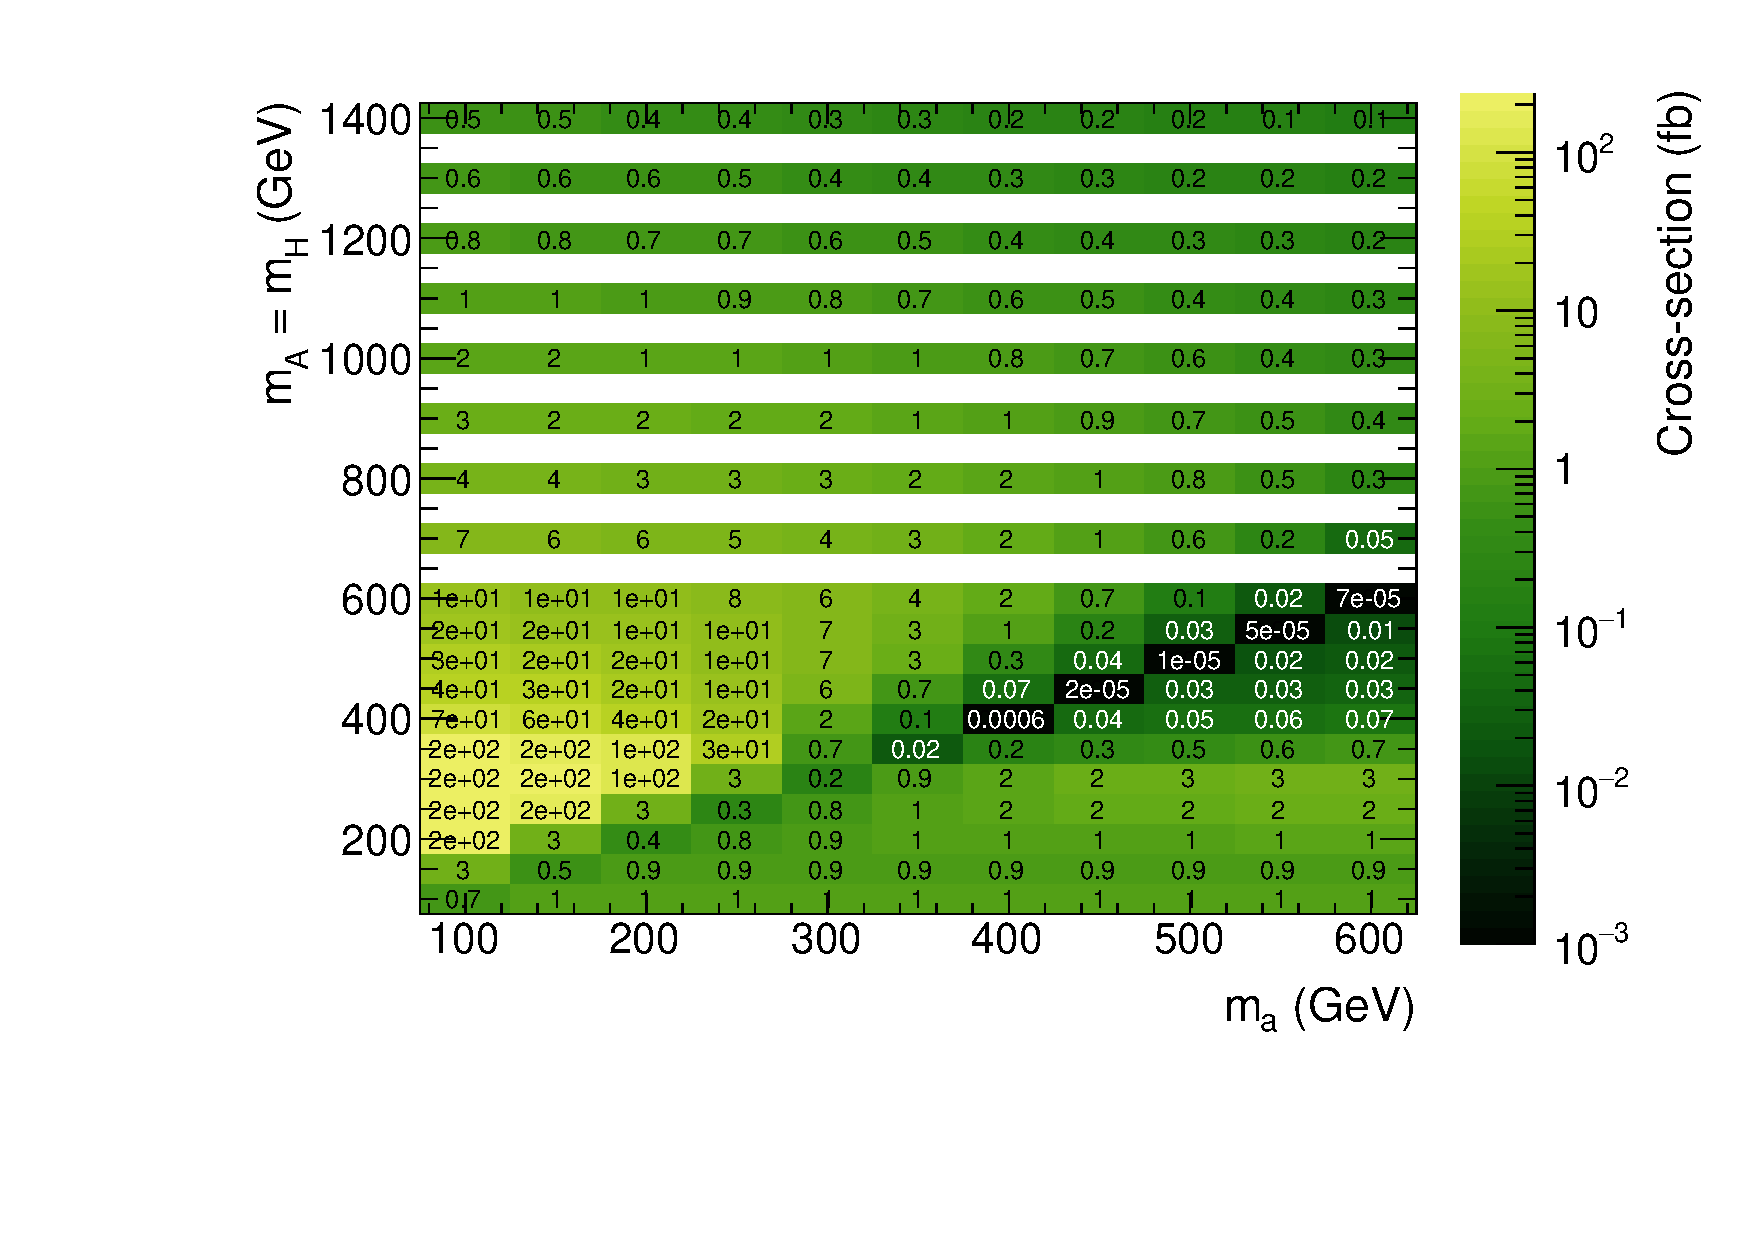
\includegraphics[width=0.8\textwidth]{texinputs/04_grid/figures/monoz/leptonic/xs_2d_inclusive_26300.pdf}
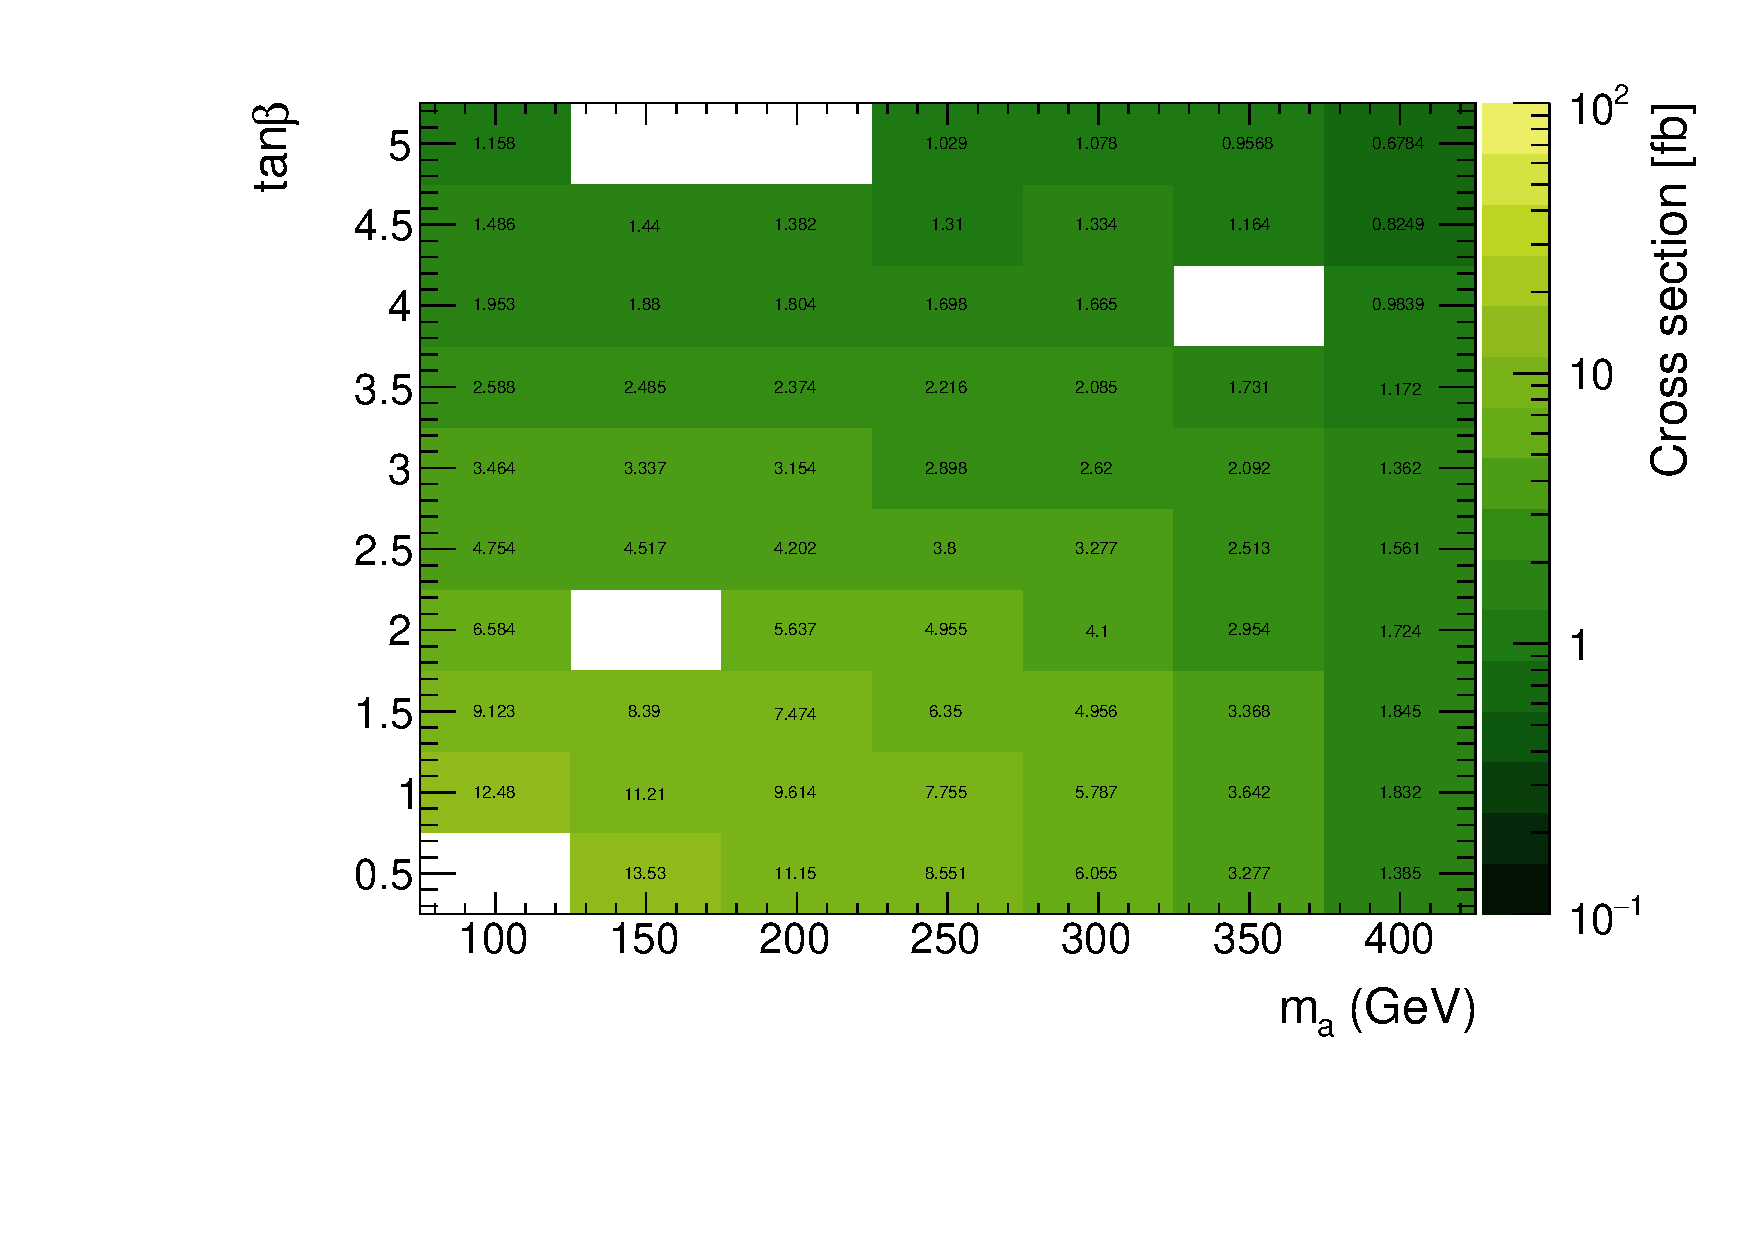
\includegraphics[width=0.8\textwidth]{texinputs/04_grid/figures/monoz/leptonic/tanbma_xsec_ll.pdf}
\caption{Inclusive cross-sections for $pp\rightarrow \lp\lm\chi\overline{\chi}$ in the \ma-\mA (top) and \ma-\tanb scans (bottom).}
\label{fig:monoz_ll_xs_inclusive}
\end{figure}

In the mass scan, maximal cross-sections are observed for the region of $\ma < \mA$ for values of $\ma\gtrsim100$ GeV. Towards higher values of both \ma and \mA, the cross-sections fall off, reaching values smaller than $1$ fb at $\ma\approx450$ GeV or $\mA\approx1.1$ TeV. In the $\ma\approx\mA$-region, the cross-section is suppressed by destructive interference. For the region with inverted mass hierarchy $\ma>\mA$, cross-sections of the order of multiple fb are observed, as long as $|\ma-\mA|$ remains sufficiently large.
In the \tanb scan, cross-sections smoothly fall with increasing $\ma$ as well as $\tanb$. Cross-sections are typically larger than 1 fb up to $\tanb\approx5$. The $\ma$ dependence is modulated by the value of \tanb: Crossing the $\ma$ range from $100$ to $400$ GeV, cross-sections are reduced by a factor $\approx7$ for small $\tanb\approx1$, but only a factor $\approx2$ for higher values of $\tanb\approx5$.
In the \sinp scan shown in Figure \ref{fig:monoz_ll_sinp_scan_xsec}, cross sections depends on whether or not the $a \rightarrow \ttbar$ decays are accesible.  
For $\ma < 350$ GeV they are not accesible and cross section strictly increases with \sinp.  For $\ma > 350 \GeV$, the $a \rightarrow \ttbar$ decays become possible causing the cross section to decrease for large values of \sinp.

%For \ma <350 GeV they are not accesible,  and only the heavy scalar's branching fraction to $aZ$ is relevant.  This branching fraction stricly increases with \sinp.  For \ma > 350 \GeV, the branching fraction of $a \rightarrow \chi \chi$ also becomes important, and there is a turnover point were the cross section decreases.

\begin{figure}
\centering
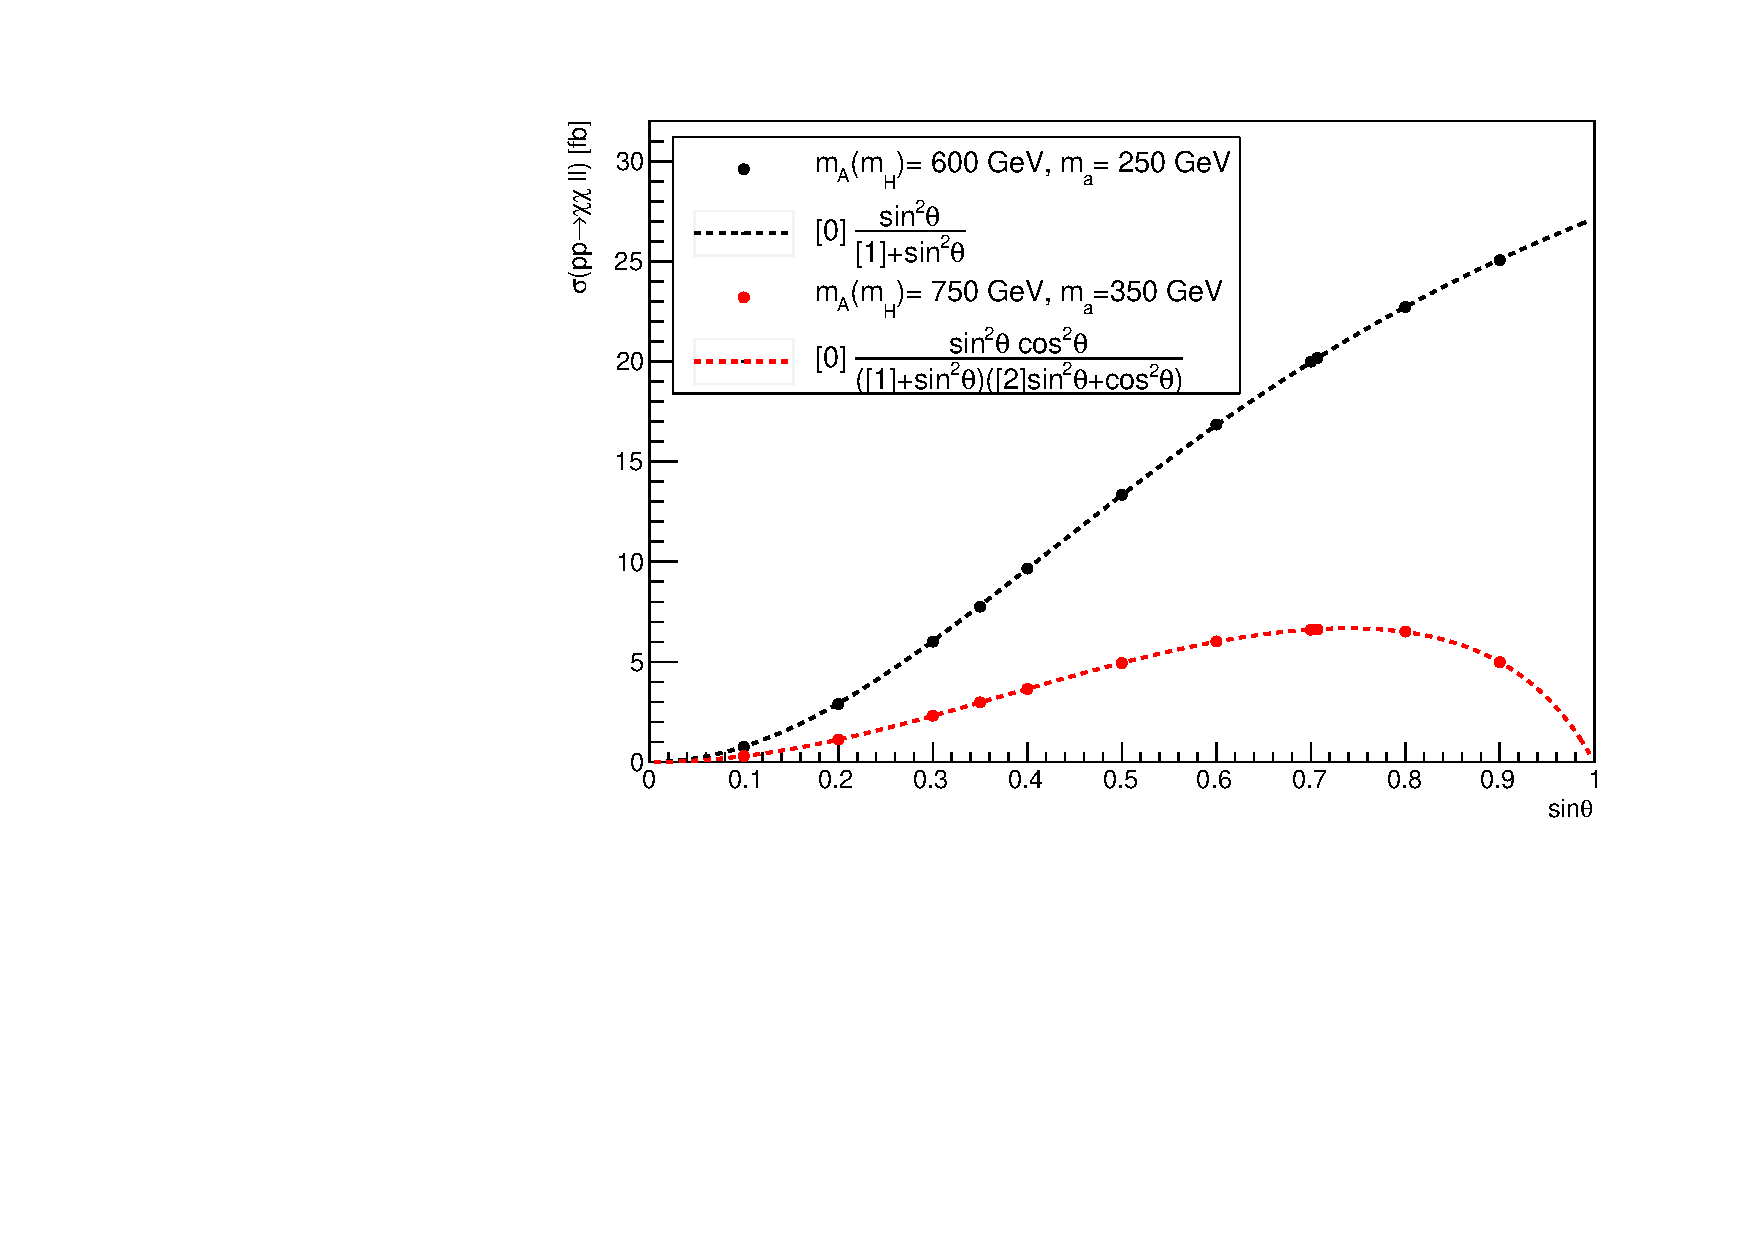
\includegraphics[width=0.6\textwidth]{texinputs/04_grid/figures/monoz/leptonic/SinThetaScan_xsecs.pdf}
\caption{For two different mass points, this figure shows the cross section $pp\rightarrow\chi\chi\ell\ell$ as a function of \sinp. 
For $\ma < 350$ GeV, $a$ decays solely to dark matter particles.  
As a consequence, the mixing angle only impacts the heavy scalar's branching fraction to $aZ$ and 
cross section strictly increases with \sinp.  
For \ma above 350 \GeV, \ttbar~ decays become accesible, introducing additional \sinp and \cosp dependences for the branching fraction 
of $a\rightarrow\chi\chi$.  For \ma above 350 GeV for large values of \sinp, there is a turnover point where the reduced $a\rightarrow\chi\chi$ branching fraction outweights the increased $H \rightarrow aZ$ branching and the net cross section decreases.}
\label{fig:monoz_ll_sinp_scan_xsec}
\end{figure}


